% !TEX root = ../Coherence.tex

\section{Introduction} 
\label{s:introduction}




%%%%%%%%%%%%%%%%%%%%%%%%%%%%%%%%


\subsection{Coherence and rewriting for monoidal categories}
We start from a set $A$, considered as a set of  ``formal generating objects"  (they are meant to be interpreted as objects in some category).  We define two sets   of object terms and morphism terms, respectively:
$$\begin{array}{l}
T::= a\  \;(\mbox{where}\;a\in A) \Alt I \Alt T\otimes T\\
M ::= \alpha \Alt \lambda \Alt\rho\Alt  \alpha^{-1} \Alt \lambda^{-1} \Alt\rho^{-1} \Alt M\comp M\Alt \id\Alt M\otimes M
\end{array}$$
In English, an object term is either a generator $a$, or $I$, or, if $S,T$ are object terms, then so is $S\otimes T$.
We actually only consider {\em well typed} morphism terms  which are the ones accepted by the following typing rules, where $M:T_1\rightarrow T_2$, called a typing assertion, should be read as ``$M$ is a morphism term with source $T_1$ and target $T_2$'':
$$\seq{}{\alpha:(T_1\otimes T_2)\otimes T_3\rightarrow T_1\otimes(T_2\otimes T_3)}\quad\quad
\seq{}{\lambda:I\otimes T\rightarrow T}\quad\quad\seq{}{\rho:T\otimes I\rightarrow T}$$
$$\seq{}{\alpha^{-1}:T_1\otimes(T_2\otimes T_3)\rightarrow (T_1\otimes T_2)\otimes T_3}\quad\quad
\seq{}{\lambda^{-1}: T\rightarrow I\otimes T}\quad\quad\seq{}{\rho^{-1}:T\rightarrow T\otimes I}$$

$$\seq{}{\id:T\rightarrow T}\quad\quad \seq{M_1:T_1\rightarrow T_2\quad M_2:T_2\rightarrow T_3}{M_2\comp M_1:T_1\rightarrow T_3}\quad\quad \seq{M_1:T_1\rightarrow T'_1\quad M_2:T_2\rightarrow T'_2}{M_1\otimes M_2:T_1\otimes T_2\rightarrow T'_1\otimes T'_2}$$
In English, each formal typing rule reads as: if all the typing assertions above the horizontal bar hold, then the typîng assertion below the bar holds.  If $M:T_1\rightarrow T_2$ is well-typed, we write $T_1={\text s}(M)$ and $T_2={\text t}(M)$. Two well typed morphism terms are called {\em parallel} it they have the same source and target.

One quotients the set of morphism terms by the laws of categories and of bifunctors, and by Mac Lane's coherence equations.
What one then obtains is the free monoidal category ${Free}(A)$ over $A$, i.e., for every {\em function} $\rho:A\rightarrow \cat{C}$ (mapping each formal generator $a$ to an object of  a monoidal category $\cat{C}$), there exists a unique {\em strict monoidal functor} $\dl \_\dr^\rho_{\cat{C}}:{Free}(A)\rightarrow\cat{C}$ that extends it.

The coherence theorem asserts that, for any two  parallel morphism terms $M,M':T\rightarrow T'$, we have $\dl M\dr^\rho_{\cat{C}}=\dl M'\dr^\rho_{\cat{C}}$  (for any monoidal category, and any valuation). An equivalent variant of this statement is limited to morphism terms which are stratified as composites (or sequences, or paths) of {\em basic} morphism terms, i.e., those terms that are formed without using composition and in which there is at most one occurrence of a constant, i.e., $\alpha,\lambda,\rho$ or their inverses. Formally, they are the terms defined by the following subsyntax:
$$B ::= \alpha \Alt \lambda \Alt\rho\Alt  \alpha^{-1} \Alt \lambda^{-1} \Alt\rho^{-1} \Alt  \id\otimes B \Alt B\otimes \id.$$
As usual, one writes also, say, $T\otimes B$ for $\id\otimes B$, when $\id:T\rightarrow T$. Alternatively, we can emphasise the unique occurrence of $\kappa\in\set{\alpha,\lambda,\rho,\alpha^{-1},\lambda^{-1},\rho^{-1}}$ in $B$ by defining a syntax of basic {\em contexts}:
$$C ::= [\,] \Alt \id\otimes C \Alt C\otimes \id.$$
We  write  $C[\kappa]$ (resp.$C[T]$) for the result of the obvious operation of filling the unique occurrence of the {\em hole} $[\,]$ with a constant $\kappa$ (resp. an object term $T$). With this notation, we see that, say, if $\alpha:(T_1\otimes T_2)\otimes T_3\rightarrow T_1\otimes(T_2\otimes T_3)$, then we have
$C[\alpha]:C[(T_1\otimes T_2)\otimes T_3]\rightarrow C[T_1\otimes(T_2\otimes T_3)]$.

Then our restricted morphism terms, viewed as {\em composable} sequences of basic terms, can be generically drawn as $$T=T_0\stackrel{C_1[\kappa_1]}{\longrightarrow} T_1 \longrightarrow\dots \longrightarrow T_{n-1} \stackrel{C_n[\kappa_n]}{\longrightarrow} T_n=T'$$
the composability assumption being that  $C_i[{\text t}(\kappa_i)]=C_{i+1}[{\text s}(\kappa_{i+1}]$, for all $i<n$.
Here is a simple illustration:
$$T_1\otimes((T_2\otimes I)\otimes T_3)\stackrel{C_1[\alpha]}{\longrightarrow}  T_1\otimes(T_2\otimes (I\otimes T_3)) 
\stackrel{C_2[\lambda]}{\longrightarrow} T_1\otimes (T_2\otimes T_3),$$
where $C_1=T_1\otimes[\,]$ and $C_2=T_1\otimes(T_2\otimes\lambda)$.
It is readily seen that any morphism term can be brought into this restricted form, so that the coherence result above can be reformulated to its more usual form that ``all diagrams commute'', where ``all'' ranges over diagrams each of whose arrows is a basic morphism term.

There are four  ingredients in Mac Lane's original proof in \cite{MacLane98}, that we recast here in the language of term rewriting theory. 
Each of the {\em non inverted} constants is a name for an associated {\em rewriting rule}, via the following dictionary:
$$\begin{array}{ccc}
\alpha & \lambda & \rho\\
(x\otimes y)\otimes z\rightarrow x\otimes(y\otimes z) & I\otimes x\rightarrow x & x\otimes I \rightarrow x.
\end{array}$$
Here $x,y,z$ stand for {\em variables}. The typing rules for $\alpha,\lambda,\rho$ provide names for the {\em instantiations} of these rewriting rules. More precisely, say,  $\alpha:(T_1\otimes T_2)\otimes T_3\rightarrow T_1\otimes(T_2\otimes T_3)$ ``is'' the instantiation of the rule $\alpha$
where $x,y,z$ are mapped to $T_1$, $T_2$, $T_3$, respectively.
Each $C[\kappa]$ is a name for a {\em rewriting step}, consisting in applying (an instance of) rule $\kappa$ in context $C$.
In the example above, we have rewritten the object term $T_1\otimes((T_2\otimes I)\otimes T_3)$ to $T_1\otimes(T_2\otimes (I\otimes T_3))$ by applying $\alpha$, instantiated at $T_1$, $(T_2\otimes I)$, $T_3$, and in context $T_1\otimes[\,]$.

The first three ingredients of Mac Lane's proof of coherence are the following.
\begin{enumerate}
\item The rewriting system defined by $\alpha,\lambda,\rho$ is strongly normalising (i.e. there is no infinite rewriting sequence).
\item All critical pairs can be solved.  We explain this notion by an example.  The term $(((x_1\otimes x_2)\otimes x_3)\otimes x_4$ can be rewritten via $\alpha$, but also via $\alpha\otimes x_4$, leading to $t_1=(x_1\otimes x_2)\otimes (x_3\otimes x_4)$ and $t_2=((x_1\otimes (x_2\otimes x_3))\otimes x_4$, respectively.  Solving the critical pair means finding a term $t$, a rewriting path from $t_1$ to $t$ and a rewriting path from $t_2$ to $t$. Applying this to the current situation, we get $t=x_1\otimes(x_2\otimes (x_3\otimes x_4))$ and
$$t_1 \stackrel{\alpha}{\longrightarrow} t \quad\quad\quad\quad t_2 \stackrel{\alpha}{\longrightarrow} (x_1\otimes ((x_2\otimes x_3)\otimes x_4) \stackrel{\alpha}{\longrightarrow} t$$
We have synthesised Mac Lane's pentagonal coherence condition! The adjective ``critical'' refers to both {\em overlapping} and {\em minimality} of the situation described above. As an example of non-overlapping, consider $(I\otimes x_1)\otimes(((x_2\otimes x_3)\otimes x_4)$ where the reductions $\lambda\otimes \id$ and $\id \otimes\alpha$ are independent and can be performed in either order, leading to a square of reductions. As an example of non-minimality, place the whole above pentagon in some non trivial context $C$, i.e., start from 
$C[(((x_1\otimes x_2)\otimes x_3)\otimes x_4]$.
\end{enumerate}
Condition (2) implies local confluence (this is known as Knuth-Bendix lemma, and is closely related to Bergman's diamond lemma), and local confluence and condition (1) imply confluence (this is known as Newman's lemma). The next ingredient is the following:
\begin{enumerate}
\item[(3)]
The proof of Newman's lemma can be upgraded to a proof of coherence for parallel paths $M,M':T\rightarrow T'$, where $M,M'$ contain no inverted constants. This is just a matter of naming the steps taken in the proof! 
\end{enumerate}
Then comes the fourth  and last ingredient.
\begin{enumerate}
\item[(4)] Coherence follows from this restricted (directed) coherence. The strategy for establishing this is to note that for fixed $T,T'$, if   there exists at least one morphism term $M:T\rightarrow T'$, then  $T$ and $T'$  have the same normal form $\tilde T$, and that for any such pair 
$T,T'$, the restricted coherence gives  us morphism terms from $T$ to $\tilde T$ and from $T'$ to $\tilde T$, depending from $T$ and $T'$ only (up to the coherence conditions). By inverting the second path and concatenating, we get a special morphism term from $T$ to $T'$ and one shows that every morphism term $M:T\rightarrow T'$ is equal to this path, modulo the coherence conditions.
\end{enumerate}
We shall expand this discussion when dealing with coherence for hypergraph polytopes obtained via rewriting techniques.

%%%%%%%%%%%%%%%%%%%%%%%%%%%%%%

\subsection{Categorified non-symmetric operads}

\begin{definition}[Categorified non-symmetric operad] A \emph{categorified non-symmetric operad} $\mathcal{P}$ is a collection $\left\{  \mathcal{P}(n)  \right\}_{n\in \mathbb{N}}$ of small categories equipped with bifunctors  
$$ \begin{array}{clll}
\circ_i&\colon& \mathcal{P}(n) \times
                  \mathcal{P}(k)
                  \longrightarrow \mathcal{P}(n+k-1) \ ,
                  & \text{for}\ 1 \leq i \leq n \ ,
\end{array}  $$
an object $\mathrm{id} \in \mathcal{P}(1)$ called \emph{unit}, and for each $\kappa \in \mathcal{P}(m)$,  $\mu \in \mathcal{P}(n)$, $\nu \in \mathcal{P}(k)$ natural isomorphisms 
$$ \begin{array}{clll}
    \beta_{\kappa,\mu,\nu}&\colon& 
    (\kappa \circ_i \mu) \circ_{j+i-1} \nu  \overset{\cong}{\longrightarrow} \kappa \circ_i (\mu \circ_j \nu) \ , &  \\
    \theta_{\kappa,\nu,\mu}&\colon& 
    (\kappa \circ_i \nu) \circ_{j+k-1} \mu 
    \overset{\cong}{\longrightarrow} (\kappa \circ_j \mu) \circ_i \nu \ , & \text{when}\ i < j \ , \\
    \lambda_\nu &\colon& 
    \mathrm{id} \circ_1 \nu \overset{\cong}{\longrightarrow} \nu \ , & \\
    \rho_\mu &\colon& 
    \mu \circ_i \mathrm{id} \overset{\cong}{\longrightarrow} \mu \ , & 
\end{array}  $$
such that the following diagrams commute: the triangle \\
\begin{center}
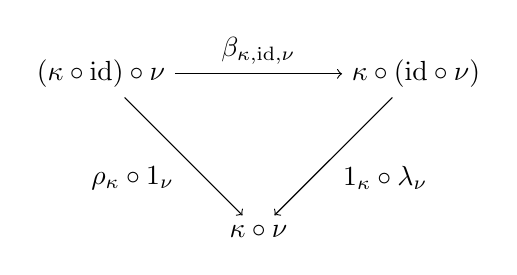
\begin{tikzpicture}[scale=2]
    \node (P1) at (-1,1) {$(\kappa \circ \mathrm{id})\circ \nu$};
    \node (P2) at (1,1) {$\kappa \circ (\mathrm{id}\circ \nu)$};
    \node (P3) at (0,0) {$\kappa \circ \nu$};
    \draw[->] (P1)--(P2) node[midway,above] {$\beta_{\kappa,\mathrm{id},\nu}$};
    \draw[->] (P1)--(P3) node[midway,below left] {$\rho_\kappa\circ 1_\nu$};
    \draw[->] (P2)--(P3) node[midway,below right] {$1_\kappa \circ \lambda_\nu$};
\end{tikzpicture} \quad \quad 
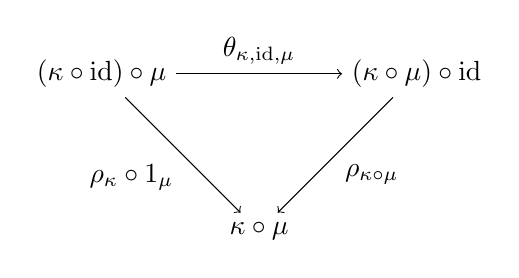
\begin{tikzpicture}[scale=2]
    \node (P1) at (-1,1) {$(\kappa \circ \mathrm{id})\circ \mu$};
    \node (P2) at (1,1) {$(\kappa\circ \mu)\circ\mathrm{id}$};
    \node (P3) at (0,0) {$\kappa \circ \mu$};
    \draw[->] (P1)--(P2) node[midway,above] {$\theta_{\kappa,\mathrm{id},\mu}$};
    \draw[->] (P1)--(P3) node[midway,below left] {$\rho_\kappa\circ 1_\mu$};
    \draw[->] (P2)--(P3) node[midway,below right] {$\rho_{\kappa\circ\mu}$};
\end{tikzpicture} \quad \ ,
\end{center}
pentagonal \\
\resizebox{\linewidth}{!}{
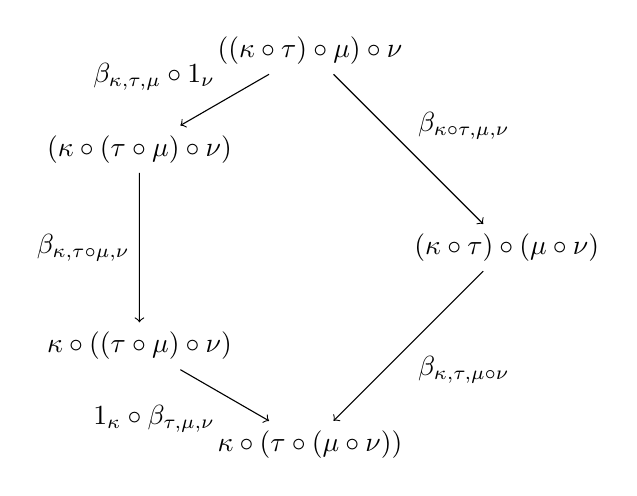
\begin{tikzpicture}[scale=2.5]
    \node (P1) at (0,1) {$((\kappa\circ\tau)\circ\mu)\circ\nu$};
    \node (P2) at (-0.866,0.5) {$(\kappa\circ(\tau\circ\mu)\circ\nu)$};
    \node (P3) at (-0.866,-0.5) {$\kappa\circ((\tau\circ\mu)\circ\nu)$};
    \node (P4) at (0,-1) {$\kappa\circ(\tau\circ(\mu\circ\nu))$};
    \node (P5) at (1,0) {$(\kappa\circ\tau)\circ(\mu\circ\nu)$} ;
    \draw[->] (P1)--(P2) node[midway,above left] {$\beta_{\kappa,\tau,\mu}\circ 1_\nu$};
    \draw[->] (P2)--(P3) node[midway,left] {$\beta_{\kappa,\tau\circ\mu,\nu}$};
    \draw[->] (P3)--(P4) node[midway,below left] {$1_\kappa \circ \beta_{\tau,\mu,\nu}$};
    \draw[->] (P1)--(P5) node[midway,above right] {$\beta_{\kappa\circ\tau,\mu,\nu}$};
    \draw[->] (P5)--(P4) node[midway,below right] {$\beta_{\kappa,\tau,\mu\circ\nu}$};
\end{tikzpicture} \quad 
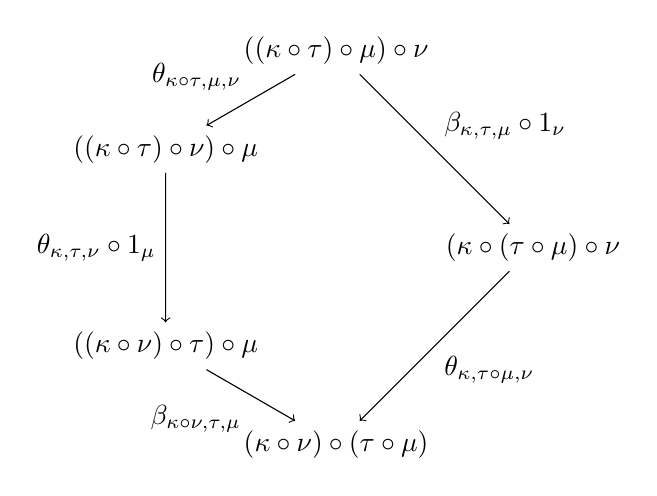
\begin{tikzpicture}[scale=2.5]
    \node (P1) at (0,1) {$((\kappa\circ\tau)\circ\mu)\circ\nu$};
    \node (P2) at (-0.866,0.5) {$((\kappa\circ\tau)\circ\nu)\circ\mu$};
    \node (P3) at (-0.866,-0.5) {$((\kappa\circ\nu)\circ\tau)\circ\mu$};
    \node (P4) at (0,-1) {$(\kappa\circ\nu)\circ(\tau\circ\mu)$};
    \node (P5) at (1,0) {$(\kappa\circ(\tau\circ\mu)\circ\nu$} ;
    \draw[->] (P1)--(P2) node[midway,above left] {$\theta_{\kappa\circ\tau,\mu,\nu}$};
    \draw[->] (P2)--(P3) node[midway,left] {$\theta_{\kappa,\tau,\nu}\circ 1_\mu$};
    \draw[->] (P3)--(P4) node[midway,below left] {$\beta_{\kappa\circ\nu,\tau,\mu}$};
    \draw[->] (P1)--(P5) node[midway,above right] {$\beta_{\kappa,\tau,\mu}\circ 1_\nu$};
    \draw[->] (P5)--(P4) node[midway,below right] {$\theta_{\kappa,\tau\circ\mu,\nu}$};
\end{tikzpicture} \quad 
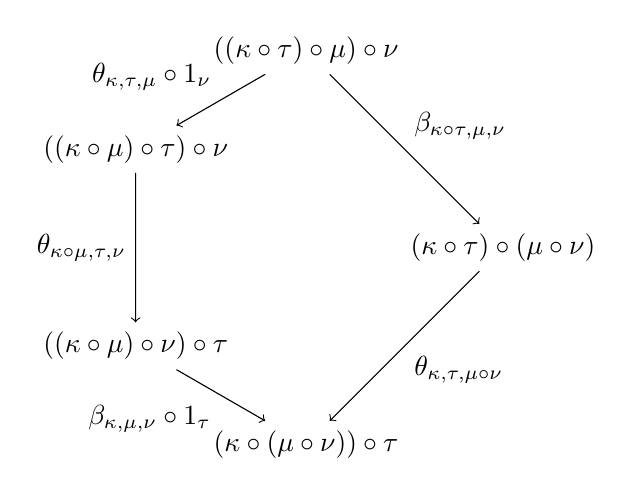
\begin{tikzpicture}[scale=2.5]
    \node (P1) at (0,1) {$((\kappa\circ\tau)\circ\mu)\circ\nu$};
    \node (P2) at (-0.866,0.5) {$((\kappa\circ\mu)\circ\tau)\circ\nu$};
    \node (P3) at (-0.866,-0.5) {$((\kappa\circ\mu)\circ\nu)\circ\tau$};
    \node (P4) at (0,-1) {$(\kappa\circ(\mu\circ\nu))\circ\tau$};
    \node (P5) at (1,0) {$(\kappa\circ\tau)\circ(\mu\circ\nu)$} ;
    \draw[->] (P1)--(P2) node[midway,above left] {$\theta_{\kappa,\tau,\mu}\circ 1_\nu$};
    \draw[->] (P2)--(P3) node[midway,left] {$\theta_{\kappa\circ\mu,\tau,\nu}$};
    \draw[->] (P3)--(P4) node[midway,below left] {$\beta_{\kappa,\mu,\nu}\circ 1_\tau$};
    \draw[->] (P1)--(P5) node[midway,above right] {$\beta_{\kappa\circ\tau,\mu,\nu}$};
    \draw[->] (P5)--(P4) node[midway,below right] {$\theta_{\kappa,\tau,\mu\circ\nu}$};
\end{tikzpicture} } \\
and hexagonal identities \\
\begin{center}
\resizebox{0.8\linewidth}{!}{
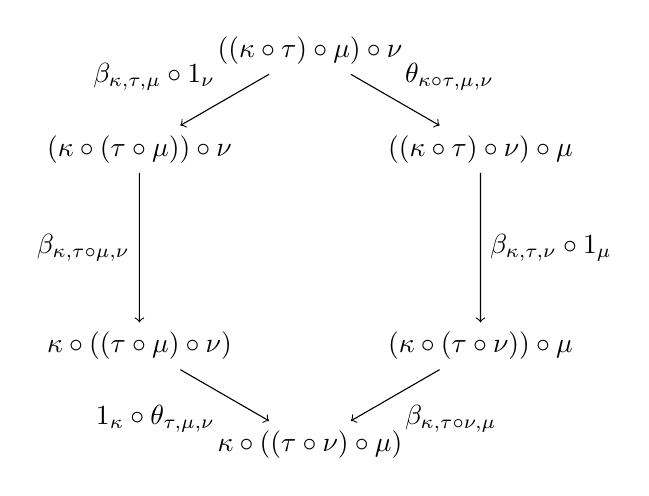
\begin{tikzpicture}[scale=2.5]
    \node (P1) at (0,1) {$((\kappa\circ\tau)\circ\mu)\circ\nu$};
    \node (P2) at (-0.866,0.5) {$(\kappa\circ(\tau\circ\mu))\circ\nu$};
    \node (P3) at (-0.866,-0.5) {$\kappa\circ((\tau\circ\mu)\circ\nu)$};
    \node (P4) at (0,-1) {$\kappa\circ((\tau\circ\nu)\circ\mu)$};
    \node (P5) at (0.866,0.5) {$((\kappa\circ\tau)\circ\nu)\circ\mu$} ;
    \node (P6) at (0.866,-0.5) {$(\kappa\circ(\tau\circ\nu))\circ\mu$};
    \draw[->] (P1)--(P2) node[midway,above left] {$\beta_{\kappa,\tau,\mu}\circ 1_\nu$};
    \draw[->] (P2)--(P3) node[midway,left] {$\beta_{\kappa,\tau\circ\mu,\nu}$};
    \draw[->] (P3)--(P4) node[midway,below left] {$1_\kappa \circ \theta_{\tau,\mu,\nu}$};
    \draw[->] (P1)--(P5) node[midway,above right] {$\theta_{\kappa\circ\tau,\mu,\nu}$};
    \draw[->] (P5)--(P6) node[midway,right] {$\beta_{\kappa,\tau,\nu}\circ 1_\mu$};
    \draw[->] (P6)--(P4) node[midway,below right] {$\beta_{\kappa,\tau\circ\nu,\mu}$};
\end{tikzpicture} \quad \quad
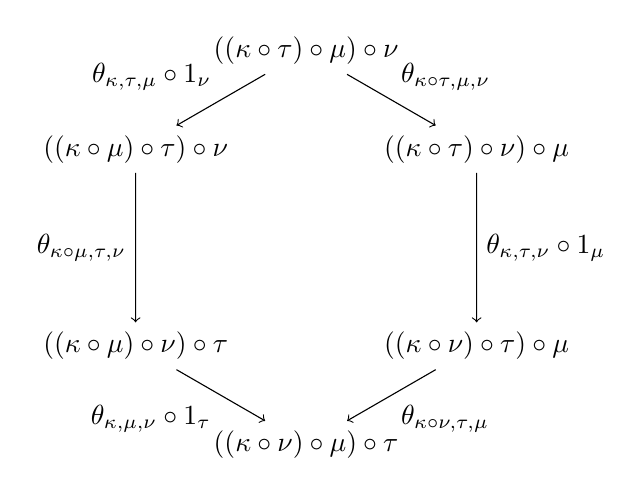
\begin{tikzpicture}[scale=2.5]
    \node (P1) at (0,1) {$((\kappa\circ\tau)\circ\mu)\circ\nu$};
    \node (P2) at (-0.866,0.5) {$((\kappa\circ\mu)\circ\tau)\circ\nu$};
    \node (P3) at (-0.866,-0.5) {$((\kappa\circ\mu)\circ\nu)\circ\tau$};
    \node (P4) at (0,-1) {$((\kappa\circ\nu)\circ\mu)\circ\tau$};
    \node (P5) at (0.866,0.5) {$((\kappa\circ\tau)\circ\nu)\circ\mu$} ;
    \node (P6) at (0.866,-0.5) {$((\kappa\circ\nu)\circ\tau)\circ\mu$};
    \draw[->] (P1)--(P2) node[midway,above left] {$\theta_{\kappa,\tau,\mu}\circ 1_\nu$};
    \draw[->] (P2)--(P3) node[midway,left] {$\theta_{\kappa\circ\mu,\tau,\nu}$};
    \draw[->] (P3)--(P4) node[midway,below left] {$\theta_{\kappa,\mu,\nu}\circ 1_\tau$};
    \draw[->] (P1)--(P5) node[midway,above right] {$\theta_{\kappa\circ\tau,\mu,\nu}$};
    \draw[->] (P5)--(P6) node[midway,right] {$\theta_{\kappa,\tau,\nu}\circ 1_\mu$};
    \draw[->] (P6)--(P4) node[midway,below right] {$\theta_{\kappa\circ\nu,\tau,\mu}$};
\end{tikzpicture}  } \quad \ .
\end{center}
\end{definition}

A categorified ns operad concentrated in arity 1 is a monoidal category.


%%%%%%%%%%%%%%%%%%%%%%%%%%%%%%%%%%%%%%%%


\subsection{Basic facts about polytopes}

Vertex figure
Every pair of edges is connected by a path

\subsection{Reminders on hypergraph polytopes}

A hypergraph is given by a set  $H$ of vertices (the carrier), and a subset 
$\hyper{H}\inc {\mathcal{P}}(H)\backslash\emptyset$ such that $\Union \hyper{H}=H$.
 The elements of $\hyper{H}$ are called the {\em hyperedges} of $\hyper{H}$.  
 We always assume that $\hyper{H}$ is {\em atomic}, by which we mean that 
 $\set{x}\in \hyper{H}$, for all $x\in H$. 
 Identifying $x$ with $\set{x}$, $H$ can be seen as the set of  hyperedges of 
 cardinality $1$, also called {\em vertices}. We shall use the convention to 
 give the same name to the hypergraph and to its carrier, in different fonts. 
 %When this convention cannot be used, we use the notation $V(\hyper{H})$ for the set of vertices of $\hyper{H}$.
% In the sequel, we shall write $\hyper{H}$ for an atomic  hypergraph, and $H$ for its set of vertices, i.e. 
%$H=\Union\hyper{H}$.
A hyperedge of cardinality 2 is called an {\em edge}.  Note that any ordinary graph $(V,E)$ can be viewed as the atomic hypergraph
$\setc{\set{v}}{v\in V} \union \setc{e}{e\in E}$ (with no hyperedges of cardinality $\geq 3$). 

\smallskip
 
If $\hyper{H}$ is a hypergraph,  and if  $X\inc H$, we set
$\hyper{H}_X:=\setc{Z}{Z\in \hyper{H}\;\mbox{and}\; Z\inc X}$, and $\restrH{H}{X}=\hyper{H}_{H\backslash X}$.
We say that $\hyper{H}$ is {\em connected} if there is no non-trivial partition $H=X_1\union X_2$ such that $\hyper{H}=\hyper{H}_{X_1}\union \hyper{H}_{X_2}$, and that $X\inc H$ is connected in $\hyper{H}$ if $\hyper{H}_X$ is connected.
%All our hypergraphs will be finite. 
For each finite hypergraph there exists a partition
$H=X_1\union\ldots\union X_m$ such that each $\hyper{H}_{X_i}$ is connected and $\hyper{H}=\Union(\hyper{H}_{X_i})$.  The $\hyper{H}_{X_i}$'s are  the {\em connected components} of $\hyper{H}$. The notation
$\hyper{H},X  \leadsto \hyper{H}_1,\ldots, \hyper{H}_n$
 will mean that  $\hyper{H}_1,\ldots,\hyper{H}_n$ are  the
 connected components of $\restrH{H}{X}$.  
%We shall  write
%$\hyper{H}_i$  for
%$\hyper{H}_{H_i}$. 

\smallskip

Do\v sen and Petri\'c~\cite{DP} have proposed the following insightful reading of the data of a finite connected hypergraph $\hyper{H}$ as a truncated simplex: the elements of $H$ are identified with the facets (i.e. codimension 1 faces) of the $(|H|-1)$-dimensional simplex, and each $\emptyset\incs X\incs H$, $|X|\geq 2$, such that    $\hyper{H}_X$ is connected designates the intersection of the facets in $X$ as a face to be truncated.
The obtained polytopes, called \emph{hypergraph polytopes}, extend the construction of graph associahedra \cite{CD-CCGA, Zel06}, and are equivalent to nestohedra, as introduced by Postnikov \cite{P09}.  Moreover,  the faces of the   polytope obtained by performing  all the prescribed truncations  are labeled by non-planar trees whose nodes are decorated by non-empty subsets of $H$, called {\em constructs}, whose recursive definition  we give next using a syntax introduced in \cite{COI}:

\smallskip
Let  $\emptyset\neq Y\subseteq H$. If   $\hyper{H},Y  \leadsto \hyper{H}_1,\ldots, \hyper{H}_n$, and if  $T_1,\ldots,T_n$ are constructs of $\hyper{H}_1,\ldots,\hyper{H}_n$, respectively, then the tree obtained by grafting $T_1,\ldots,T_n$ on the root node decorated by $Y$, denoted by $Y(T_1,\ldots,T_n)$, is a construct of  $\hyper{H}$~\footnote{\label{construct-tubing} Constructs are in one-to-one correspondence with tubings as defined in \cite{CD-CCGA}: for a given construct $T$, each tube of the associated tubing is given by a node of $T$ and all its descendance. There are  as many tubes in the tubing as nodes in the construct.}. We write $Y=\mbox{root}(Y(T_1,\ldots,T_n))$.

\smallskip
 The base case is when $Y=H$ (and hence $n=0$): then the one-node tree $H()$ (written simply $H$) is a construct.
We write $T:\hyper{H}$ to denote that $T$ is a construct of $\hyper{H}$. 
The formalism of constructs   allows us to view the inclusion of faces of a hypergraph polytope through the process of contracting tree edges: by contracting an edge of a construct and  merging the decorations of the two nodes related by that edge, one gets a covering construct.

\smallskip
Simplices are ``encoded'' as the hypergraphs  $$\hyper{S}^X=\setc{\set{x}}{x\in X}\union\set{\set{X}}$$ (no truncation prescribed). The constructs have the form $Y(\ldots,\set{y},\ldots)$ where $\emptyset\incs Y\inc X$ and $y$ ranges over $H\backslash Y$, and are therefore isomorphic to multipointed sets. In order to illustrate  how the hypergraph structure dictates truncations, consider the hypergraph $\hyper{H}=\set{\set{x},\set{y},\set{z},\set{y,z}, \set{x,y,z}}$, obtained from $\hyper{S}^{\{x,y,z\}}$ by adding the edge $\{y,z\}$. The construct 
 $\set{x}(\set{y},\set{z}):\hyper{S}^{\{x,y,z\}}$ is {\em not} a construct of $\hyper{H}$, since $\hyper{H}_{\set{y,z}}$ is connected.  Instead, $\hyper{H}$ features 3 new constructs: 
$\set{x}(\set{y}(\set{z}))$, $\set{x}(\set{z}(\set{y}))$ and $\set{x}(\set{y,z})$, encoding two  vertices and one edge, obtained by truncating  the vertex $\set{x}(\set{y},\set{z})$ of $\hyper{S}^{\{x,y,z\}}$.

As a slightly more involved example, we show in Figure \ref{hemiassoc} the polytope encoded by the hypergraph $\hyper{H}=\{\{x\},\{y\},\{u\},\{v\},\{x,y\},\{x,u\},\{x,v\},\{u,v\},\{x,u,v\}\}$, obtained from the  tetrahedron by truncating three of its vertices and four of its edges. We also ``zoom in'' into the square obtained by the truncation prescribed by $\{u,v\}$  and label its four 1-dimensional and four 0-dimensional faces by the appropriate constructs of $\hyper{H}$. 

% !TEX root = ../Coherence.tex

\begin{figure}
\centering
  \resizebox{4cm}{!}{
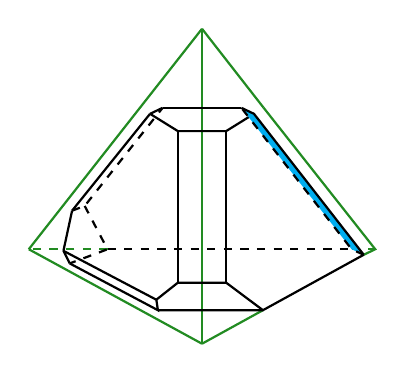
\begin{tikzpicture}[thick,scale=2]
\coordinate (A1) at (0,2);
\coordinate (A11) at (-0.39,1.5);
\coordinate (A111) at (-0.25,1.498);
\coordinate (A112) at (-0.33,1.46);
\coordinate (A12) at (0.39,1.5);
\coordinate (A121) at (0.25,1.498);
\coordinate (A122) at (0.33,1.46);
\coordinate (A13) at (0,1.25);
\coordinate (A131) at (-0.153,1.35); 
\coordinate (A132) at (0.153,1.35); 
\coordinate (A2) at (0,0); 
\coordinate (A21) at (-0.387,0.213); 
\coordinate (A211) at (-0.29,0.2795); 
\coordinate (A212) at (-0.28,0.213); 
\coordinate (A22) at (0.387,0.213); 
\coordinate (A23) at (0,0.5); 
\coordinate (A231) at (-0.153,0.388); 
\coordinate (A232) at (0.153,0.388); 
\coordinate (A3) at (-1.1,0.6);
\coordinate (A31) at (-0.9,0.49);
\coordinate (A311) at (-0.88,0.59);
\coordinate (A312) at (-0.84,0.51);
\coordinate (A32) at (-0.8,0.976);
\coordinate (A321) at (-0.825,0.845);
\coordinate (A322) at (-0.745,0.875);
\coordinate (A33) at (-0.6,0.6);
\coordinate (A4) at (1.1,0.6);
\coordinate (A41) at (1.027,0.565);
\coordinate (A42) at (0.95,0.6);
%\draw[draw=none,fill=cyan!40,opacity=0.5] (A42)--(A41)--(A121)--(A122)-- cycle;
\draw[draw=ForestGreen]  (A3)--(A2);
\draw[draw=ForestGreen]  (A1)--(A12);
\draw[draw=ForestGreen] (A2)--(A22);
\draw[draw=ForestGreen] (A2) -- (A1);
\draw[draw=ForestGreen] (A3)--(A1);
\draw[draw=ForestGreen,dashed]  (A33) -- (A3);
\draw[draw=ForestGreen,dashed]  (A42) -- (A4);
\draw[draw=ForestGreen] (A41)--(A4)--(A12);
 \draw[draw=black,fill=none]   (A321)--(A311);
 \draw[draw=black,fill=none] (A212)-- (A22) -- (A41);
\draw (A311)--(A312);
\draw (A111)--(A121);
\draw (A111)--(A112);
\draw (A311)--(A211)--(A212) --(A312);
\draw (A112)--(A321);
\draw[dashed] (A321)--(A322)--(A111);
\draw  (A211)--(A231)--(A232)--(A22);
\draw[dashed]  (A33) -- (A42);
\draw (A231) -- (A131) -- (A132) -- (A232) -- cycle;
\draw[dashed] (A322) -- (A33) -- (A312);
\draw (A112) -- (A131) --(A132)--(A122);
\fill[cyan] (A41) -- (A42) -- (A121)--(A122)--cycle;
\draw[dashed]  (A41) -- (A42) -- (A121); 
\draw (A41)--(A122) --(A121);
\end{tikzpicture}} \quad\quad  
\raisebox{1em}{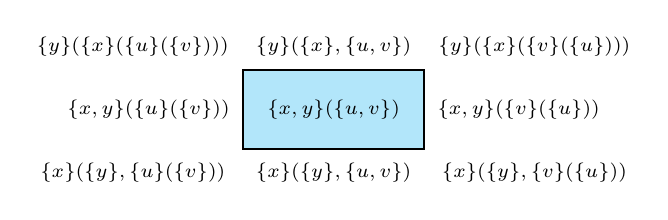
\begin{tikzpicture}[thick]
\coordinate (S1) at (-0.15,0);
\coordinate (S2) at (2.15,0);
\coordinate (S3) at (2.15,1);
\coordinate (S4) at (-0.15,1);
\draw[fill=cyan,opacity=0.3] (S1)--(S2)--(S3)--(S4)-- cycle;
\draw (S1)--(S2)--(S3)--(S4)-- cycle;
\node (s1) at (-1.55,-0.3) {\scriptsize $\{x\}(\{y\},\{u\}(\{v\}))$};
\node (s2) at (3.55,-0.3) {\scriptsize $\{x\}(\{y\},\{v\}(\{u\}))$};
\node (s4) at (-1.55,1.3) {\scriptsize $\{y\}(\{x\}(\{u\}(\{v\})))$};
\node (s3) at (3.55,1.3) {\scriptsize $\{y\}(\{x\}(\{v\}(\{u\})))$};
\node (s14) at (-1.35,0.5) {\scriptsize $\{x,y\}(\{u\}(\{v\}))$};
\node (s23) at (3.35,0.5) {\scriptsize $\{x,y\}(\{v\}(\{u\}))$};
\node (s12) at (1,-0.3) {\scriptsize $\{x\}(\{y\},\{u,v\})$};
\node (s34) at (1,1.3) {\scriptsize $\{y\}(\{x\},\{u,v\})$};
\node (s) at (1,0.5) {\scriptsize $\{x,y\}(\{u,v\})$};

\end{tikzpicture}}
\caption{A truncated simplex. \label{hemiassoc}}
\end{figure}

We recover associahedra and permutohedra as  linear and complete graphs, respectively: 

$$\begin{array}{ll}
\hyper{K}^X= \set{\set{x_1},\ldots,\set{x_n},\set{x_1,x_2},\ldots,\set{x_{n-1},x_n},\set{x_1,\ldots x_n}}, \\
\hyper{P}^X= \set{\set{x_1},\ldots,\set{x_n},\set{x_1,\ldots x_n}} \cup \setc{\set{x_i,x_j}}{1\leq i\neq j\leq n},
\end{array}$$



